% Paper template for TAR 2022
% (C) 2014 Jan Šnajder, Goran Glavaš, Domagoj Alagić, Mladen Karan
% TakeLab, FER

\documentclass[10pt, a4paper]{article}
\usepackage{tar2023}
\usepackage{float}
\usepackage[utf8]{inputenc}
\usepackage[pdftex]{graphicx}
\usepackage{booktabs}
\usepackage{amsmath}
\usepackage{amssymb}
\usepackage{url} 

\title{Ideology and Power Identification in Parliamentary Debates}

\name{Medved Fran, Šarić Dominik, Topić Karla} 

\address{
University of Zagreb, Faculty of Electrical Engineering and Computing\\
Unska 3, 10000 Zagreb, Croatia\\ 
\texttt{fran.medved@fer.hr, dominik.saric@fer.hr, karla.topic@fer.hr}\\
}
          
         
\abstract{ 
This document provides the instructions on formatting the TAR system description paper in \LaTeX{}. This is where you write the abstract (i.e., summary) of the work you carried out within the project. The abstract is a paragraph of text ranging between 70 and 150 words.
}

\begin{document}

\maketitleabstract

\section{Introduction}

In modern democratic societies, debates within national parliaments play a crucial role, not only shaping the lives of citizens withing a country, but often exerting influence on a global scale. These debates serve as a fundamental platform for political discourse, shaping public policy and reflecting the ideological and power dynamics within the political landscape.

However, the language used in parliamentary speeches is often complex and indirect, posing significant challenges for computational analysis. Traditionally, political scientists and analysts have manually analyzed and classified parliamentary speeches. They carefully review and interpret each speech to determine the speaker's political orientation and affiliations. Although this method is thorough, it is very time-consuming and cannot keep up with the large amount of data produced in modern parliamentary sessions. But, recent advancements in natural language processing (NLP) provide promising tools to address this challenge, particularly through the use of Recurrent Natural Networks (RNNs) and Transformer models. 

This research leverages the strengths of Transformer models to predict ideological orientation in parliamentary debates. The baseline models include Linear Classifier with Gradient Descent (SGD), RNN, and Transformer models, which will be compared with a newly proposed Recursive Transformer (RTransformer) and Linear (RLinear) model. This model processes entire text sequences, converts words into embeddings, and applies transformer encoding with recursive reduction to capture hierarchical data structures. By training these model on a dataset of parliamentary speeches, the study aims to develop a robust system capable of automatically identifying the political leanings of speakers based on their speech content.

By automating the identification of political ideology, we can provide political analysts and researchers with powerful tools to efficiently process and interpret large volumes of speech data.

\section{Related Work}

Iyyer et al. (2014) applied recursive neural networks (RNNs) to detect ideological bias in text by using the hierarchical nature of language. Their model constructs a parse tree where each word in a sentence is represented by a vector, and these vectors are recursively combined to form phrase and sentence-level representations. This approach allows the model to capture ideological bias that emerges from the composition of words and phrases. Building on the same foundational idea of using parse trees to capture hierarchical structures, our research utilizes the recursive approach with a Transformer model rather than the RNN. This allows us to harness the power of self-attention mechanisms in Transformers, which can weigh the importance of each word in the context of the entire sequence.

Baly et al. (2020) investigated how to predict political ideology in news articles by using both Long Short-Term Memory networks (LSTMs) and Bidirectional Encoder Representations from Transformers (BERT). They faced a significant challenge: models often picked up on the writing styles of specific news outlets instead of the political biases within the articles themselves. To overcome this, they introduced adversarial media adaptation and triplet loss pre-training. These techniques helped the models focus more on the ideological content rather than just stylistic elements.

Kulkarni et al. (2018) proposed a multi-view model for detecting political ideology in news articles by incorporating cues from title, link structures and content. This attention-based model significantly outperformed the state-of-the-art models by incorporating network structures and content cues. Their approach underlines the importance of using diverse features beyond textual content alone to enhance the detection of ideological bias.

These studies collectively demonstrate significant advancements in the field of political ideology detection, each contributing unique methodologies and datasets that enhance our understanding of ideological bias in text. Building on these foundations, our research aims to leverage the strengths of recursive transformers to classify ideology in parliamentary debates.

\section{Methodology}

\subsection{Dataset Description}
\label{sec:first}

The dataset for this study is derived from the ParlaMint project, a multilingual and comparable corpus of parliamentary debates \citep{parlamint-2021}. Each entry in the dataset includes the transcribed speech text in English and a binary label indicating political orientation (0 for left-wing, 1 for right-wing). The dataset is specifically trained on speeches from Croatia, ensuring a focused and representative sample.

\subsection{Preprocessing}
Preprocessing steps were applied to the dataset to enhance model performance. Two versions of the dataset were created: one with stopwords removed and another with stopwords retained. This dual approach enables a comparison of the models to assess the impact of preprocessing.
Text normalization was performed by converting all text to lowercase to ensure consistency. For stopword removal, the spaCy library was utilized, which efficiently identifies and eliminates stopwords from the text (spaCy, 2021).

\subsection{Linear Classifier with Gradient Descent} 

The Linear Classifier with Gradient Descent is a supervised learning model used for classification tasks. It employs the Stochastic Gradient Descent (SGD) algorithm to optimize the log loss (logistic loss) function, finding the best decision boundary that separates data points of different classes. For the baseline in this study, the Linear Classifier with Gradient Descent is employed to classify the political orientation of parliamentary speeches.

\subsection{Recurrent Neural Network} 

The Recurrent Neural Network (RNN) used in this study is designed to classify the political orientation of parliamentary speeches. This bidirectional RNN processes input sequences in both forward and backward directions, allowing it to capture the full context of each word. The model consists of four RNN layers with a hidden dimension of 600, followed by a ReLU activation and two fully connected layers. The final output is transformed into a probability using the sigmoid function.

RNN provides a robust baseline for comparing the performance of more advanced models such as Transformers and the proposed Recursive Transformer model.

\subsection{Transformers} 

The Transformer model is designed to handle sequential data, making it highly effective for natural language processing tasks. Unlike traditional RNNs, Transformers use self-attention to process all tokens in a sequence simultaneously, capturing long-range dependencies more efficiently.

The model includes an embedding layer to convert input sequences into vectors and positional encodings to maintain word order. It consists of multiple Transformer encoder layers with multi-head self-attention and feed-forward networks. The output is pooled and passed through fully connected layers to produce a final probability using the sigmoid function. This Transformer model provides a strong baseline for classifying the political orientation of parliamentary speeches since our own proposed model will be based on the transformers architecture.

\subsection{Proposed Model: Recursive Transformer} 

The Recursive Transformer (RTransformer) is the proposed model for classifying the political orientation of parliamentary speeches. This model builds on the standard Transformer architecture, incorporating recursion to handle hierarchical structures within the data more effectively. 

The entire text from a single row in dataset is treated as a one input, with each word in the text being converted into an embedding, providing a dense representation of the word's meaning. Data is processed in batches with padding to ensure uniform input lengths. For each position \textit{t}, the kernel captures a phrase of \textit{k} word embeddings. The Transformer encoder then processes this phrase to produce a phrase-level representation:
\[
h_{t} = \text{TransformerEncoder}(x_{t:t+k})
\]
where \(\mathit{x}_{t:t+k}\) denotes the sequence of \textit{k} word embeddings starting at position \textit{t}. The stride \textit{s} determines the next starting position for the kernel, summarizing information in overlapping windows as it moves through the text. For subsequent layers, these phrase-level representations are recursively encoded:
\[
h_{t+1} = \text{TransformerEncoder}(h_{t})
\]
Each recursive step reduces the sequence length by summarizing information. Finally, once the sequence is reduced to a single representation, a linear transformation followed by a sigmoid function is applied to generate the final classification output:
\[
\hat{y} = \sigma(W_{\text{class}} \cdot h_{\text{final}} + b)
\]
where \( W_{\text{class}} \) is the weight matrix for the classification layer, \( h_{\text{final}} \) is the final hidden state of the Transformer encoder, and \( \sigma \) is the sigmoid function. The sigmoid function is defined as:

\[
\sigma(z) = \frac{1}{1 + e^{-z}}
\]
The model is trained using the binary cross-entropy with logits loss function (\texttt{BCEWithLogitsLoss}), which combines a sigmoid layer and the binary cross-entropy loss in one single class. The loss function is defined as:

\[
L = -\frac{1}{N} \sum_{i=1}^{N} \left[ y_{i} \log(\sigma(z_{i})) + (1 - y_{i}) \log(1 - \sigma(z_{i})) \right]
\]
where \( y_{i} \) is the true label, \( z_{i} \) is the raw output (logit) of the model, and \( N \) is the number of samples.


By processing the entire text and reducing the sequence length through recursive steps, the RTransformer can capture long-range dependencies and hierarchical structures within the data, providing a robust solution for political orientation classification.

\subsection{Proposed Model: Recursive Linear} 

To compare the effectiveness of the RTransformer, a Recursive Linear Model (RLinear) was also implemented. The methodology for the RLinear model follows the same process as the RTransformer, with the key difference being the use of a linear model instead of a Transformer encoder at each step. This substitution allows direct comparison between two models, highlighting the impact of using a Transformer encoder versus a linear model in capturing hierarchical structures and long-range dependencies in the text. 

\section{Results}
\begin{table}[H]
\caption{Results for validation data which is not processed}
\label{tab:not processed data}
\begin{center}
\begin{tabular}{llccc}
\toprule
Model & Acc & Prec & Rec & F1 \\
\midrule
SGD & & & & \\
RNN & & & & \\
Transformer & & & & \\
RTransformer & & & & \\
RLinearModel & & & & \\
\bottomrule
\end{tabular}
\end{center}
\end{table}

\begin{table}[H]
\caption{Results for validation data which is processed}
\label{tab:processed data}
\begin{center}
\begin{tabular}{llccc}
\toprule
Model & Acc & Prec & Rec & F1 \\
\midrule
SGD & & & & \\
RNN & & & & \\
Transformer & & & & \\
RTransformer & & & & \\
RLinearModel & & & & \\
\bottomrule
\end{tabular}
\end{center}
\end{table}

\section{Conclusion}

Conclusion is the last enumerated section of the paper. It should not exceed half of a column and is typically split into 2--3 paragraphs. No new information should be presented in the conclusion; this section only summarizes and concludes the paper.

\section{Referencing literature}

ParlaMint. (2021). A multilingual comparable corpora of parliamentary debates. Retrieved from: https://www.clarin.eu/parlamint.

spaCy. (2021). spaCy: Industrial-Strength Natural Language Processing in Python. Retrieved from: https://spacy.io/.

\section*{Acknowledgements}

If suitable, you can include the \textit{Acknowledgements} section before inserting the literature references  in order to thank those who helped you in any way to deliver the paper, but are not co-authors of the paper.

References to other publications should be written in brackets with the last name of the first author and the year of publication, e.g., \citep{chomsky-73}.  Multiple references are written in sequence, one after another, separated by semicolon and without whitespaces in between, e.g., \citep{chomsky-73,chave-64,feigl-58}. 

This is the second subsection of the second section. Referencing the (sub)sections in text is performed as follows: ``in Section~\ref{sec:first} we have shown \dots''

References are typically written at the end of the sentence and necessarily before the sentence punctuation.

If the publication is authored by more than one author, only the name of the first author is written, after which abbreviation \emph{et al.}, meaning \emph{et alia}, i.e.,~and others is written as in \citep{johnson-etc}. If the publication is authored by only two authors, then the last names of both authors are written \citep{johnson-howells}.

If the name of the author is incorporated into the text of the sentence, it should not be in the brackets (only the year should be there). E.g.,~``\citet{chomsky-73}
suggested that \dots''. The difference is whether you reference the publication or the author who wrote it. 

The list of all literature references is given alphabetically at the end of the paper. The form of the reference depends on the type of the bibliographic unit: conference papers,
\citep{chave-64}, books \citep{butcher-81}, journal articles
\citep{howells-51}, doctoral dissertations \citep{croft-78}, and book chapters \citep{feigl-58}. 

All of this is automatically produced when using BibTeX. Insert all the BibTeX entries into the file \texttt{tar2023.bib}, and then reference them via their symbolic names.

\section{Figures and tables}

\subsection{Figures}

Here is an example on how to include figures in the paper. Figures are included in \LaTeX{} code immediately \textit{after} the text in which these figures are referenced. Allow \LaTeX{} to place the figure where it believes is best (usually on top of the page of at the position where you would not place the figure). Figures are referenced as follows: ``Figure~\ref{fig:figure1} shows \dots''. Use tilde (\verb.~.) to prevent separation between the word ``Figure'' and its enumeration. 

\begin{figure}
\begin{center}
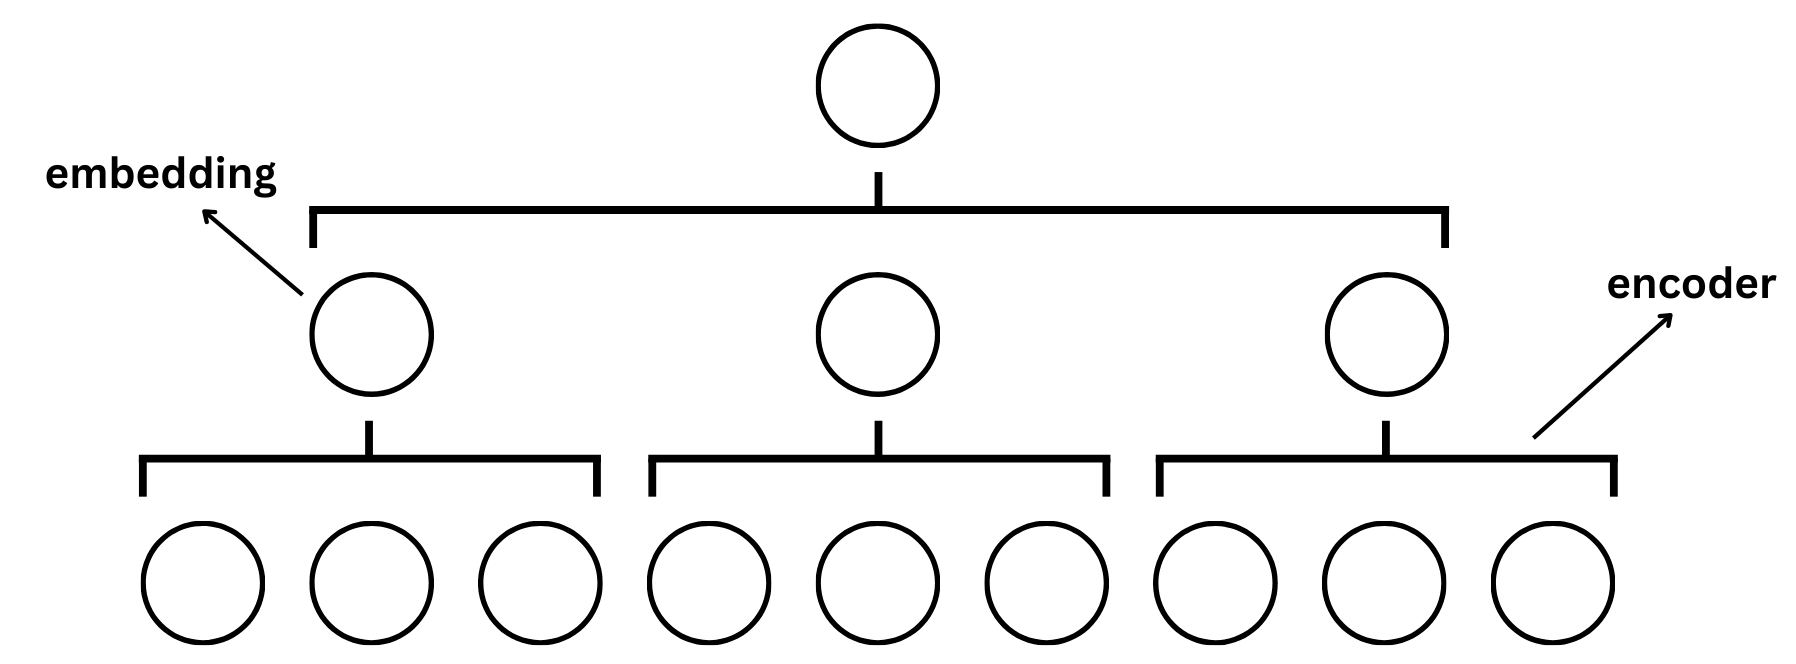
\includegraphics[width=\columnwidth]{images/RTransformer.png}
\caption{This is the figure caption. Full sentences should be followed with a dot. The caption should be placed \textit{below} the figure. Caption should be short; details should be explained in the text.}
\label{fig:figure1}
\end{center}
\end{figure}

\subsection{Tables}

There are two types of tables: narrow tables that fit into one column and a wide table that spreads over both columns.

\begin{table}
\caption{This is the caption of the table. Table captions should be placed \textit{above} the table.}
\begin{center}
\begin{tabular}{ll}
\toprule
Heading1 & Heading2 \\
\midrule
One & First row text \\
Two   & Second row text \\
Three   & Third row text \\
      & Fourth row text \\
\bottomrule
\end{tabular}
\end{center}
\end{table}

\section{Math expressions and formulas}

Math expressions and formulas that appear within the sentence should be written inside the so-called \emph{inline} math environment: $2+3$, $\sqrt{16}$, $h(x)=\mathbf{1}(\theta_1 x_1 + \theta_0>0)$. Larger expressions and formulas (e.g., equations) should be written in the so-called \emph{displayed} math environment:

\[
b^{(i)}_k = \begin{cases}
1 & \text{if 
    $k = \text{argmin}_j \| \mathbf{x}^{(i)} - \mathbf{\mu}_j \|,$}\\
0 & \text{otherwise}
\end{cases}
\]

Math expressions which you reference in the text should be written inside the \textit{equation} environment:

\begin{equation}\label{eq:kmeans-error}
J = \sum_{i=1}^N \sum_{k=1}^K 
b^{(i)}_k \| \mathbf{x}^{(i)} - \mathbf{\mu}_k \|^2
\end{equation}

Now you can reference equation \eqref{eq:kmeans-error}. If the paragraph continues right after the formula

\begin{equation}
f(x) = x^2 + \varepsilon
\end{equation}

\noindent like this one does, use the command \emph{noindent} after the equation to remove the indentation of the row. 

Multi-letter words in the math environment should be written inside the command \emph{mathit}, otherwise \LaTeX{} will insert spacing between the letters to denote the multiplication of values denoted by symbols. For example, compare
$\mathit{Consistent}(h,\mathcal{D})$ and\\
$Consistent(h,\mathcal{D})$.

If you need a math symbol, but you don't know the corresponding \LaTeX{} command that generates it, try
\emph{Detexify}.\footnote{\texttt{http://detexify.kirelabs.org/}}

\bibliographystyle{tar2023}
\bibliography{tar2023} 

\end{document}

